\section{Il modello client/server}
Al livello applicativo sono generati i messaggi da scambiare tra i calcolatori, come per esempio richieste e risposte HTTP, un protocollo associato ai browser web, messaggi di posta elettronica, o porzioni di video. I messaggi generati dall'applicazione vengono passati al livello di trasporto, che può suddividerli in segmenti e aggiungere intestazioni contenenti informazioni di controllo come il numero di sequenza. Le sezioni devono poi selezionare il servizio del livello di trasporto, tra: \begin{itemize}
	\item \textbf{Protocollo TCP}: Servizio orientato alla connessione il quale garantisce la consegna dell'informazione.
	\item \textbf{Protocollo UDP}: Servizio non orientato alla connessione il quale non garantisce la consegna dell'informazione.
\end{itemize}
\noindent Applicazioni diverse hanno necessità di servizi diversi. Per esempio, un client di posta elettronica richiede che ogni informazione sia consegnata al destinatario; di conseguenza userà un protocollo che si appoggia alla garanzia di consegna del TCP, come \textbf{SMTP}.\par
Invece, un sito web come Twitch fornisce un contenuto "Tollerante alle perdite", quindi se non tutti i dati sono consegnati non necessariamente l'esperienza sarà danneggiata. Per esempio durante una livestream è richiesto di mantenere una connessione in tempo reale, privilegiando la continuità della riproduzione rispetto alla completa affidabilità dei dati, accettando eventuali ritardi o perdite limitate.\par
La "selezione del servizio" per l'invio di un messaggio si traduce in termini di apertura di un \textbf{socket} verso la destinazione, ovvero un'astrazione software che rappresenta il punto di accesso tra applicazione e livello di trasporto. Per aprirne uno è necessario specificare \textbf{protocollo} di trasporto, \textbf{indirizzi IP} di sorgente e destinazione e \textbf{porta} di sorgente e destinazione, le quali identificano l'interfaccia. I due processi che comunicano con il socket si identificano nei ruoli di: \begin{itemize}
	\item \textbf{Client}: Processo che inizia la comunicazione.
	\item \textbf{Server}: Il processo in attesa di contatto; accetta le richieste di comunicazione.
\end{itemize}
\noindent È un errore comune quello di confondere l'host con il client. Sebbene spesso un host coincida con un singolo client o server, una macchina può eseguire contemporaneamente più processi, assumendo quindi entrambi i ruoli.

\begin{figure}[h]
	\centering
	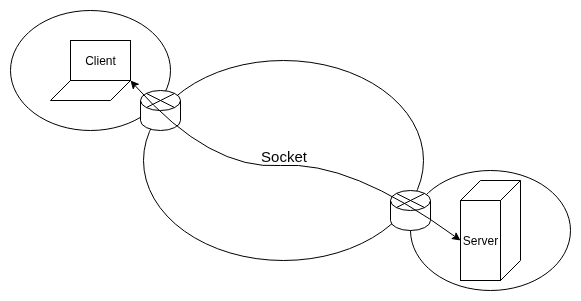
\includegraphics[width=0.8\linewidth]{Images/socket.png}
	\caption{Apertura di un socket}
\end{figure}

%

\section{Hyper Text Transfer Protocol - HTTP}
\textbf{HTTP} è un protocollo a livello di applicazione del Web implementato in due processi client e server, i quali comunicano mediante uno scambio di messaggi HTTP. Il protocollo definisce struttura e modalità di scambio dei messaggi e si serve di \textbf{pagine Web}, generalmente costituite da un file HTML (Hypet Text Markup Language) principale detto \textbf{index.html} entro il quale si referenziano gli \textbf{oggetti}; file indirizzabili tramite URL come immagini, file JS o un foglio di stile CSS.\par
Il lato client del protocollo è implementato da un \textbf{browser Web}, come Firefox, per l'invio delle richieste, mentre il server è gestito dal \textbf{Web server}, il quale ospita gli oggetti menzionati prima. Quando un utente richiede una pagina Web, il browser invia al server messaggi di \textbf{richiesta HTTP} per ottenere gli oggetti nella pagina; si riceve quindi una \textbf{risposta HTTP}, la quale può essere positiva, confermando che il trasferimento degli oggetti è andato a buon fine, oppure negativa se la pagina non è stata trovata o è inesistente.\par
HTTP si appoggia al protocollo di trasporto TCP; infatti, il client stabilisce in primo luogo una connessione TCP con il server, alla quale i processi accedono tramite le proprie socket. Inoltre, il server invia i file richiesti senza memorizzare alcuna informazione di stato del client; per questa ragione diciamo che HTTP è un protocollo \textbf{senza memoria di stato}.

\begin{figure}[h]
	\centering
	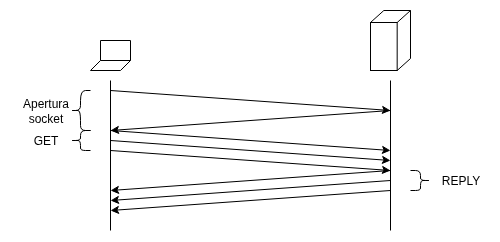
\includegraphics[width=0.8\linewidth]{Images/basicHTTP_get-reply.png}
	\caption{Protocollo HTTP}
\end{figure}

\noindent Presentiamo ora la struttura dei messaggi di richiesta e risposta HTTP. Il primo è composto da più righe: la prima è detta \textbf{riga di richiesta} e presenta tre campi: \begin{itemize}
	\item \textbf{Metodo}: Indica la procedura da attuare, come GET per richiedere risorse, POST per inviare informazioni al server, o DELETE, per cancellare informazioni sul server.
	\item \textbf{URL}: Identifica gli oggetti sui quali usare il metodo.
	\item \textbf{Versione HTTP}: Indica la versione del protocollo utilizzata.
\end{itemize}
\noindent Le righe successive sono dette di \textbf{intestazione} e tutte tranne quella che indica l'host (nella versione 1.1) sono opzionali. Determinano dati diversi come il browser utilizzato o la lingua del messaggio da inviare, come anche il tipo di connessione. Segue esempio: \begin{verbatim}
	GET /index.html HTTP/1.1
	Host: www.univr.it
	Connection: close
	User-agent: Mozilla/4.0
	Accept-language: it
\end{verbatim}
\noindent I messaggi di risposta HTTP presentano invece tre sezioni: una \textbf{riga di stato} iniziale, delle \textbf{righe di intestazione} e il \textbf{corpo}, contenente la risorsa richiesta.\par
La prima riga è composta a sua volta da tre campi: la versione del protocollo, il codice di stato e il suo corrispettivo messaggio di stato, come [200-OK], [400-Bad request] o [404-Not found]. Le successive righe invece indicano molte informazioni come, tra l'altro, il tipo di connessione, la data e l'ora di ottenimento e invio della risorsa, il nome del web server e la data e l'ora dell'ultima modifica della risorsa. Segue esempio: \begin{verbatim}
	HTTP/1.1 200 OK
	Connection: close
	Date: Thu, 18 Aug 2020 15:44:04 GMT
	Server: Apache/2.2.3 (CentOS)
	Last-Modified: Tue, 18 Aug 2020 15:11:03 GMT
	Content-Length: 3164
	Content-Type: text/html
	(Contenuto della risorsa...)
\end{verbatim}
\noindent Nella creazione delle applicazioni web gli sviluppatori devono fare una scelta: inviare le coppie richiesta/risposta su connessioni TCP separate o sulla stessa? Il primo approccio si realizza con \textbf{connessioni non persistenti}, mentre il secondo con le \textbf{persistenti}. Sono entrambe scelte valide e funzionali, sebbene di default, HTTP implementi la seconda modalità.\par
Supponiamo di avere una connessione non persistente e che un client richieda le risorse di una pagina web con 10 immagini JPEG. In sequenza, avviene: \begin{enumerate}
	\item Client HTTP inizializza una connessione TCP con il server sulla porta 80, default per HTTP. Associate alla connesione ci sono due socket: uno per il client, l'altro per il server.
	\item Il Client HTTP invia tramite il socket una richiesta HTTP al server.
	\item Il Server HTTP riceve il messaggio del client, recupera l'oggetto dalla propria memoria e lo incapsula in una risposta HTTP per inviargliela tramite il socket.
	\item Il Server HTTP comunica a TCP di terminare la connessione, cosa che avviene una volta consegnato il messaggio intero al client.
	\item Il Client riceve la risposta, estrae il file dal messaggio e lo esamina, trovando i riferimenti alle immagini JPEG.
	\item I primi quattro passi sono ripetuti per ogni oggetto da recuperare.
\end{enumerate}
\noindent Essendo che si apre e chiude una connessione TCP per ogni risorsa da recuperare, avremo un totale di 11 connessioni. Queste possono essere settate per lavorare sequenzialmente o in parallelo.\par
A partire da HTTP 1.1 sono state introdotte le connessioni persistenti, dove il server mantiene la connessione TCP aperta anche dopo l'invio di tutte le risorse. Si possono inviare intere pagine web in una volta, come anche più pagine web, allo stesso client. La connessione ha termine quando rimane inattiva per un dato lasso di tempo configurabile.\newline

\noindent Come già menzionato, i server HTTP sono privi di stato, per rendere lo sviluppo di applicazioni più semplice e con prestazioni migliori. Tuttavia, accade spesso di dover autenticare gli utenti, per ragioni di sicurezza e per fornire contenuti in funzione della loro identità. I \textbf{cookies} servono esattamente a questi scopi: consentono ai server di tener conto degli utenti.\par
Al primo utilizzo della pagina web, il server crea un codice associato all'utente che verrà inviato nella reply HTTP con l'header \textbf{SET COOKIE}. Il client, se accetta, memorizzerà l'indirizzo web e lo associerà al codice ricevuto. Nelle successive interazioni, se i cookie sono stati accettati, all'invio della GET da parte del client sarà presente anche un campo con il codice del cookie, il quale verrà elaborato dal server per fornire una risposta ritagliata per l'utente, a prescindere dall'indirizzo IP con il quale si collega.\newline

\noindent Un'altra importante entità di rete è la \textbf{web cache}, nota anche come proxy server. Si pone nel percorso fra client e web server e soddisfa richieste HTTP al posto di quest'ultimo con lo scopo di aumentare le prestazioni. Diminuisce infatti il ritardo di accesso alle risorse più utilizzate e di consegna dei messaggi; come conseguenza diretta, il carico di rete è nettamente diminuito.\par
Senza web cache, avremmo una situazione nella quale più utenti in una rete richiedono una stessa risorsa, più si sperimenterà un ritardo. Se invece l'architettura di rete la comprende, si presenterebbe il seguente scenario: \begin{enumerate}
	\item Browser stabilisce una connessione TCP col proxy server e invia una richiesta HTTP per la risorsa.
	\item Il proxy controlla la presenza di una copia della risorsa all'interno della propria memoria. Se è rilevata, la ritorna al client, altrimenti si apre una connessione TCP con il web server di origine per ottenerla.
	\item Quando il proxy riceve l'oggetto, ne salva una copia in memoria e ne invia un'altra al browser web.
\end{enumerate}
\noindent In genere le cache riescono a soddisfare il 70-80\% delle richieste, ma usando un server diverso da quello originale si pone il problema dell'attualizzazione dei dati. Se una risorsa è modificata nel server originale, questa non è automaticamente inviata al proxy. La soluzione alla questione si presenta nella forma del \textbf{get condizionale}: una richiesta get-HTTP con una riga di intestazione \textbf{if-modified-since}. Fondamentalmente, il browser effettua la richiesta specificando una data, ed è ricevuta dal proxy. Questo comunicherà con il web server che ritornerà la risorsa se è stata modificata entro la data specificata all'inizio. Se non ha subito modifiche, il proxy può inviarlo direttamente, altrimenti la risorsa deve essere ripresa dal web server originale.

\begin{figure}[h]
	\centering
	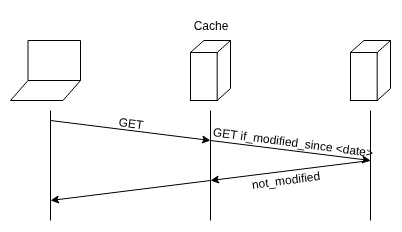
\includegraphics[width=0.5\linewidth]{Images/webCache.png}
	\caption{Web caching}
\end{figure}

%

\section{Domain Name Service - DNS}
Il servizio di directory di Internet \textbf{Domain Name Service} (DNS) ha lo scopo primario di tradurre i nomi di dominio associati ad un indirizzo IP per ritornare quest'ultimo e renderlo leggibile ai calcolatori. Si tratta in primo luogo di un database di server distribuito a livello mondiale implementato con una logica gerarchica e in secundis è un protocollo a livello di applicazione che consente agli host di interrogare la base di dati. In particolare, poggia su UDP e usa la porta 53; viene spesso utilizzato da altri protocolli a livello di applicazione, come HTTP e SMTP.\par
Supponiamo adesso che un web browser richieda la traduzione del nome di dominio "www.google.it". Il funzionamento del DNS segue le seguenti fasi: \begin{enumerate}
	\item Il calcolatore dell'utente esegue il lato client dell'applicazione DNS.
	\item Il browser estrae il nome dell'host dall'URL e lo passa al lato client dell'applicazione DNS.
	\item Il client DNS invia una \textbf{DNS query} contenente questo nome al server DNS.
	\item Il server DNS ritorna l'indirizzo IP corrispondente al dominio ricevuto.
	\item Ricevuto l'indirizzo IP, il browser web può adesso instaurare una connessione TCP verso il processo server collegato alla porta 80 di quell'indirizzo IP.
\end{enumerate}
\noindent Come si può intuire, questa procedura introduce un ritardo, ma è comune che l'indirizzo IP desiderato si trovi all'interno di server DNS cache vicini, con lo scopo di ridurre il traffico in rete e il ritardo del servizio.\par
Il DNS offre anche altri servizi, come quello di \textbf{host} e \textbf{mail aliasing}, la possibilità di usare un insieme di nomi logici dal valore equivalente (sinonimi) per ricondursi ad uno stesso host, e la \textbf{distribuzione del carico di rete}, perché è possibile replicare su più web server uno stesso nome di dominio particolarmente richiesto, al quale è associato un insieme di indirizzi IP; quando richiesto dalla query, il DNS server risponderà con l'intero insieme di indirizzi variando l'ordinamento a ogni risposta.\newline

\noindent Come già detto, più server DNS sono distribuiti per il mondo attraverso un \textbf{sistema gerarchico}; supponendo che un web browser effettui una DNS query, si esplorerebbero nel seguente ordine le tipologie dei server DNS: \begin{enumerate}
	\item \textbf{Server radice}: Contengono un insieme di indirizzi dei server TLD.
	\item \textbf{Server Top-level domain}: Si occupano dei domini di primo livello come com, it, org e simili. Forniscono gli indirizzi IP dei server autoritativi.
	\item \textbf{Server DNS autoritativi}: Appartenenti alle organizzazioni, specificano il loro dominio, come google, univr e simili.
\end{enumerate}
\noindent Infine, le organizzazioni posseggono dei \textbf{server DNS locali}, i cui indirizzi IP si possono ottenere tramite una richiesta di protocollo DHCP.\par
La distribuzione dei DNS server risolve in particolare il problema del sovraccarico, distribuendo il traffico di query, e quello della disponibilità del servizio, poiché in caso di mancata risposta da parte di un server è possibile interrogarne un altro dello stesso livello.

\begin{figure}[h]
	\centering
	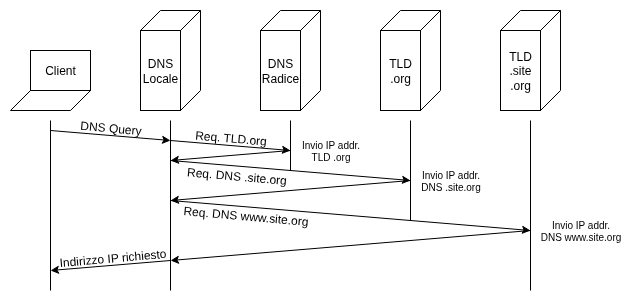
\includegraphics[width=0.75\linewidth]{Images/DNS_search.png}
	\caption{Ricerca del DNS}
\end{figure}

%

\section{Posta elettronica - SMTP e IMAP}
La posta elettronica è un mezzo di comunicazione asincrono che consente agli utenti di inviare e ricevere messaggi testuali; le e-mail moderne presentano inoltre altri oggetti, come \textbf{allegati}, \textbf{collegamenti ipertestuali}, \textbf{foto incorporate} e testo con \textbf{formattazione HTML}. Il meccanismo funziona grazie a tre elementi principali: \begin{itemize}
	\item \textbf{User agent}: Conosciuti anche come mail client, consentono di leggere, rispondere, inoltrare, salvare e comporre i messaggi. Esempi pratici sono Outlook, Gmail o Tutamail.
	\item \textbf{Mail server}: Costituiscono la parte centrale dell'infrastruttura del servizio; una casella di posta contiene i messaggi ricevuti alla quale è possibile accedere tramite autenticazione. Presenta inoltre una coda dei messaggi dove si trattengono quelli non ancora inviati.
	\item \textbf{Protocollo SMTP}: Il principale protocollo a livello di applicazione su Internet; si affida al TCP per trasferire i messaggi.
\end{itemize}
\noindent Lo scambio di messaggi tra due utenti vede generalmente una comunicazione diretta tra i due mail server; ciò significa che non sono utilizzati server intermedi, e se quello del destinatario è spento, si riproverà a inviare la mail. In condizioni ideali, invece, segue sei fasi: \begin{enumerate}
	\item L'utente A invoca il proprio user agent e fornisce l'indirizzo di posta elettronica dell'utente B. Compone il messaggio e dà istruzione allo user agent di inviarlo.
	\item Lo user agent dell'utente A invia il messaggio al suo mail server, dove è collocato in una coda di messaggi.
	\item Il lato client di SMTP, eseguito sul server dell'utente A, vede il messaggio in coda e apre una connessione TCP sulla porta 25 verso un server SMTP in esecuzione sul mail server dell'utente B.
	\item Dopo un SMTP-handshake, il client SMTP invia il messaggio dell'utente A sulla connessione TCP instaurata.
	\item Presso il mail server dell'utente B, il lato server di SMTP riceve il messaggio e lo posiziona nella casella postale.
	\item Quando ritenuto opportuno, l'utente B potrà aprire e leggere la mail invocando il proprio user agent che userà il relativo protocollo di lettura. Ad oggi è spesso usato IMAP, altrimenti sono diffuse interfacce user agent basate su HTTP.
\end{enumerate}

\begin{figure}[h]
	\centering
	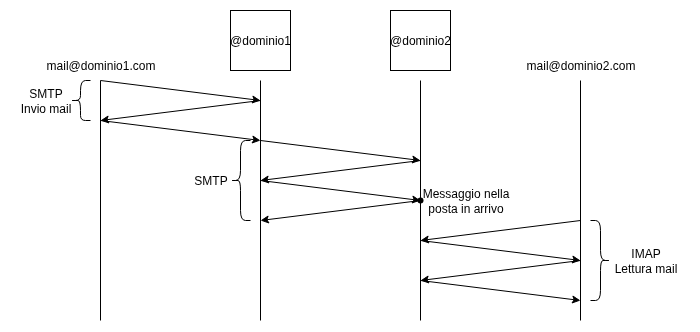
\includegraphics[width=1\linewidth]{Images/mail_exchange.png}
	\caption{Invio e ricezione posta elettronica}
\end{figure}